\section{Prepoznavanje naredbi i aktivacija zadatka}
\label{sec:prepoy}

Ako se mreža aktivira dovoljno često, za očekivati je da će najvjerojatniji izlaz iz 
neuronske mreže u slučaju izgovorene naredbe biti upravo kategorija koja predstavlja tu naredbu. 
Štoviše, naredba bi trebala biti prepoznata u više uzastopnih iteracija aktiviranja mreže.
Međutim, ponašanje sustava u tom slučaju neće biti onakvo kakvo bi trebalo, a to je da se
određeni posao (zadatak) aktivira isključivo jednom za jednom izgovorenu naredbu. 
Još jedna stvar na koju treba pripaziti je slučajno aktiviranje nekog posla jer zbog
nesavršenosti mreže se može dogoditi da vjerojatnosni izlaz ukazuje na prepoznavanje neke
naredbe iako se u stvarnosti nije izgovorila ista. Međutim, u takvim situacijama se očekuje možda jedna ili dvije takve situacije zaredom,
a ne više njih. Zbog svega navedenog, potrebno je na neki način obraditi tok vjerojatnosnih
izlaza iz neuronske mreže. Kao najbolji način za pokrivanje svih problema pokazalo se 
uprosječivanje vjerojatnosti pojedinih kategorija. 

Na slici \ref{pic:uml} prikazan je UML dijagram implementiranog podsustava. Upravljački dio posla
obavlja se unutar razreda \texttt{CommandRecognizer} koji je zadužen za aktiviranje obavljanja 
konkretnog posla koji je povezan s govornom naredbom. 
Sadrži listu pokazivača na objekte čiji razredi implementiraju 
sučelje \texttt{Command}. \texttt{Command} predstavlja sučelje (apstraktni razred) što znači da
nije moguće konstruirati objekt tog razreda, nego da je potrebno naslijediti razredom koji 
implementira apstraktnu metodu \texttt{virtual void execute(float probability)}. Ta 
metoda je zadužena za obavljanje konkretnog zadatka. Ovakav strukturni
obrazac daje mogućnost vrlo lakog implementiranja novih vrsta zadataka (sve što je potrebno je 
napraviti novi razred koji implementira sučelje \texttt{Command}, tj. nadjačava
spomenutu metodu). Trenutačno su implementirane
dvije vrste naredbi (zadataka): \texttt{BlankCommand} koja ne radi ništa (koristi se za kategorije
"pozadina" i "nepoznato") i \texttt{PrintCommand} koja ispisuje ime naredbe i prosječnu 
vjerojatnost pojavljivanja naredbe.

\begin{figure}[htb]
    \centering
    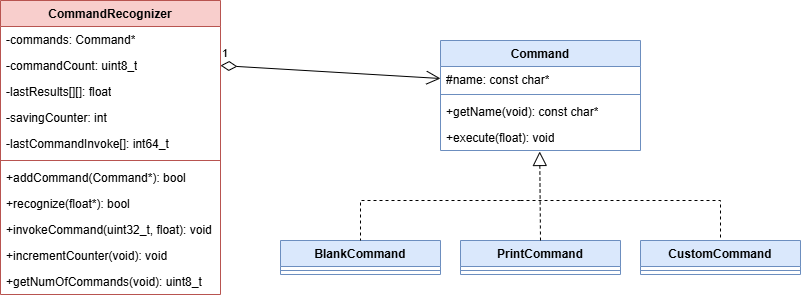
\includegraphics[width=0.9\linewidth]{Chapters/struktura_sustava/prepoznavanje_naredbi/commands.png} 
    \caption{Podsustav za prepoznavanje naredbi i aktivaciju zadataka\cite{flowchart}}
    \label{pic:uml}
\end{figure}

Prilikom konstrukcije objekta razreda koji implementira sučelje \texttt{Command} potrebno je postaviti
parametre za prepoznavanje naredbe (oni se utvrđuju eksperimentalno). Parametrom \texttt{historySize}
bira se broj uzastopnih vrijednosti vjerojatnosti pojave naredbe nad kojima se računana prosjek,
a parametar \texttt{threshold} postavlja prag koji prosječna vrijednost mora prijeći kako bi se naredba
aktivirala. Ovim se postiže odvojeno kalibriranje parametara za svaku naredbu (potrebno
je zbog podataka nad kojima se mreža uči te se zbog toga može dogoditi da se određene
naredbe prepoznaju lakše ili teže od drugih).
Uz to, objekt razreda \texttt{CommandRecognizer} brine o tome da se naredba aktivira
samo ako je prošlo određeno vrijeme nakon zadnje aktivacije. To se postiže parametrom 
\texttt{COOL\_DOWN\_PERIOD\_MS} koji je definiran u datoteci Configuration.hpp \ref{add:config}.
Jednom konstruirani objekt naredbe potrebno je dodati 
u objekt klase CommandRecognizer metodom \texttt{bool addCommand(Command* command)} 
kako bi on bio svjestan postojanja te naredbe (broj izlaza iz neuronske mreže mora odgovarati 
broju dodanih naredbi ovim putem). Svaka konkretna implementacija metode 
\texttt{virtual void execute(float probability)} ne smije trajati predugo jer će unijeti 
kašnjenje u cjelokupni sustav. Ideja je da takva naredba samo pokrene duži posao za koji će onda
biti zadužen neki drugi sustav.

U ovom trenutku opisana je cjelokupna petlja mikrokontrolerskog sustava
koja se neprestano iznova izvršava (slika \ref{pic:struktura_sustava}).
Jedina stvar koja je dosad uzimana kao "crna kutija" je sama neuronska mreža koja
je u biti okosnica cijelog sustava. Sljedeće poglavlje posvećeno je upravo njoj.